% !TEX root =  ./main.tex

\section{Toy Example}\label{sec:student}

To illustrate some basic concepts of RSs and, in the next section, of the proposed encoding, we model a system composed of a student and a vending machine as a toy example.
The vending machine accepts two different kinds of coins and can dispense either a cappuccino or an expresso when a coffee coin is inserted or a tea if a tea coin is inserted. A cappuccino is dispensed if some milk is available, otherwise expresso is produced.
Assuming the powder for preparing coffee and tea are always present, the corresponding process can be written as follows:
\[
\begin{array}{lll}
\mathsf{VM} & \triangleq & (\{\ccoin,\cpowder\},\{\nomilk\},\{\cappuccino\})\\
& | & (\{\ccoin,\cpowder,\nomilk\},\emptyset,\{\espresso\})\\
& | & (\{\tcoin,\tpowder\},\emptyset,\{\tea\})\\
& | & (\{\cpowder\},\emptyset,\{\cpowder\})\\
& | & (\{\tpowder\},\emptyset,\{\tpowder\})\\
\end{array}
\]

A refill context process can, nondeterministically, refill the machine with milk.
\[
\begin{array}{lll}
\mathsf{Refill} & \triangleq & \{\nomilk\}.\mathsf{Refill}\\
& + & \emptyset.\mathsf{Refill}\\
\end{array}
\]

The student process is very simple: she takes cappuccino in the morning and tea in the afternoon, otherwise she gets angry.
\[
\begin{array}{rll}
\mathsf{Student} & \triangleq & (\{\am\},\emptyset,\{\ccoin\}).\mathsf{GetCappuccino}\\
& + & (\emptyset,\{\am\},\{\tcoin\}).\mathsf{GetTea}\\
& + & \{\idle\}.\mathsf{Student}\\
\mathsf{GetCappuccino} & \triangleq & (\{\cappuccino\},\emptyset,\emptyset).\mathsf{Student}\\
& + & (\{\espresso\},\emptyset,\{\anger\}).\mathsf{Student}\\
\mathsf{GetTea} & \triangleq & (\{\tea\},\emptyset,\emptyset).\mathsf{Student}\\
& + & (\emptyset,\{\tea\},\{\anger\}).\mathsf{Student}\\
\end{array}
\]

Finally, two more reactions model the passage of time (morning vs afternoon) while the student is idle (i.e., not in the process of getting beverages).
\[
\begin{array}{lll}
\mathsf{Day} & \triangleq & (\{\idle\},\{\am\},\{\am\})\\
& | & (\{\am\},\{\idle\},\{\am\})
\end{array}
\]

We assume that, initially, both entitities $\cpowder$ and $\tpowder$ are present.
So the system can be written as 
\(
[\,\mathsf{Refill}
| \mathsf{Student}
| \{\cpowder,\tpowder\} 
| \mathsf{VM}
| \mathsf{Day}\,]
\).


Using BioReSolve, we can generate the underlying LTS as in Fig.~\ref{fig:toylts}: the initial state is in light blue, while the state where the student is angry is in light coral.
Note that, as \am is initially not present, it means that the initial time is in the afternoon.
To improve readability, the nodes of the LTS are labelled by the list of context processes and entities, omitting reactions, and the arcs are labelled by the the list of currently available entities, either taken from the result set or provided by the context, i.e., the components in $D\cup C$ extracted from the full label $\obs{\obs{D}{R',I',C}}{R,I,P}$. The label $0$ stands for the emptyset.
As a general strategy for BioReSolve, we use a special entity named $\Forbidden$ to mark unwanted states: here the entity is produced thanks to the auxiliary reaction $(\{\anger\},\emptyset,\{\Forbidden\})$.

\begin{figure}
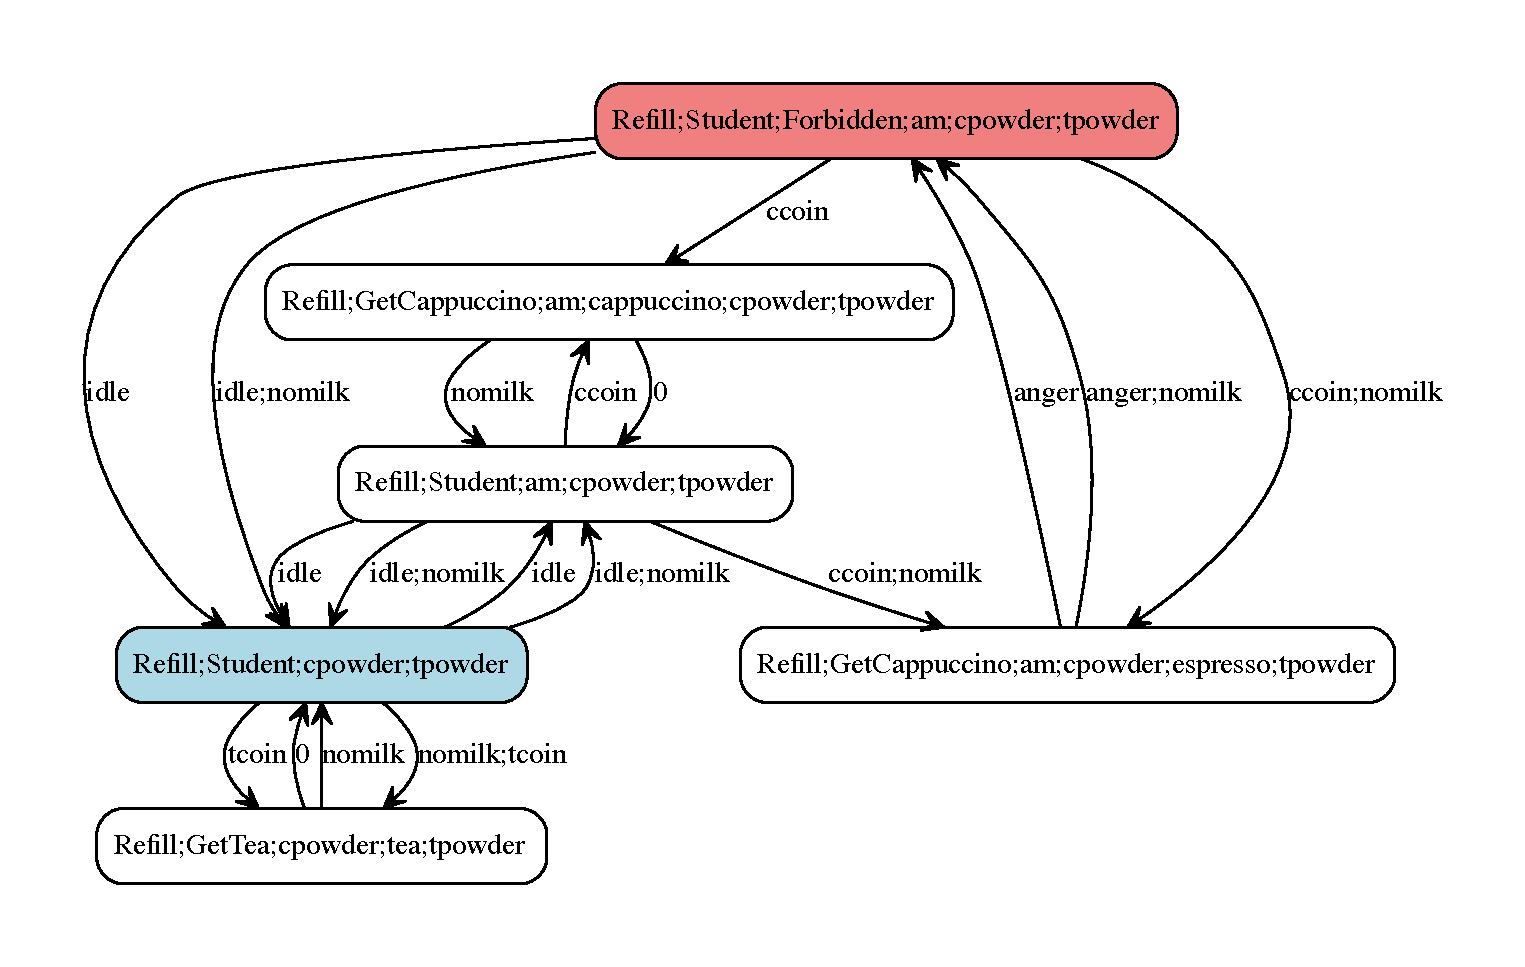
\includegraphics[scale=.3]{./figs/toylts}
\caption{LTS of the toy example.\label{fig:toylts}}
\end{figure}

By manual inspection we can recover a trace starting from the initial state and leading to the forbidden state, e.g., $\xrightarrow{\idle}\xrightarrow{\ccoin;\nomilk}\xrightarrow{\anger}$. From this trace, using the dynamic slicing process described in~\cite{DBLP:journals/nc/BrodoBF24}, we can reconstruct that the production of $\Forbidden$ was due to the prior production of $\anger$, which in turn was caused by the student getting espresso instead of cappuccino, which is because there was $\nomilk$ when a $\ccoin$ was inserted at $\am$.
